\subsection{Einleitung}
\label{sub:einleitung}
Als Projekt während der PeP et al. Sommerakademie 2013 wurde ein Solarofen gefertigt. 
In diesem Ofen sollten allein durch Sonneneinstrahlung möglichst hohe Temperaturen erreicht werden.
Ziel war es, einen Ofen zu fertigen, in dem zumindest einfache Kochaktivitäten ausgeführt werden konnten, wie beispielsweise das Kochen eines Eies oder das Backen eines kleinen Brotes.

\subsection{Theorie} 
\label{sub:theorie}
Ansatz des Solarofens ist es, Wärmeenergie ins Innere des Ofens zu führen und dort zu halten. 
Diese Energie sollte ausschließlich durch Sonneneinstrahlung gewonnen werden.
Es gilt deshalb, die Intensität des in den Ofen einfallenden Lichtes über Reflexion zu maximieren und die vom Ofen nach außen emittierte Wärmestrahlung durch Isolation zu minimieren.
Auf diese Weise soll die effektive Einstrahlfläche des Ofens vergrößert und eine zu starke Abgabe der Energie an die Umgebung vermieden werden.

\subsection{Aufbau}
\begin{figure}
\centering
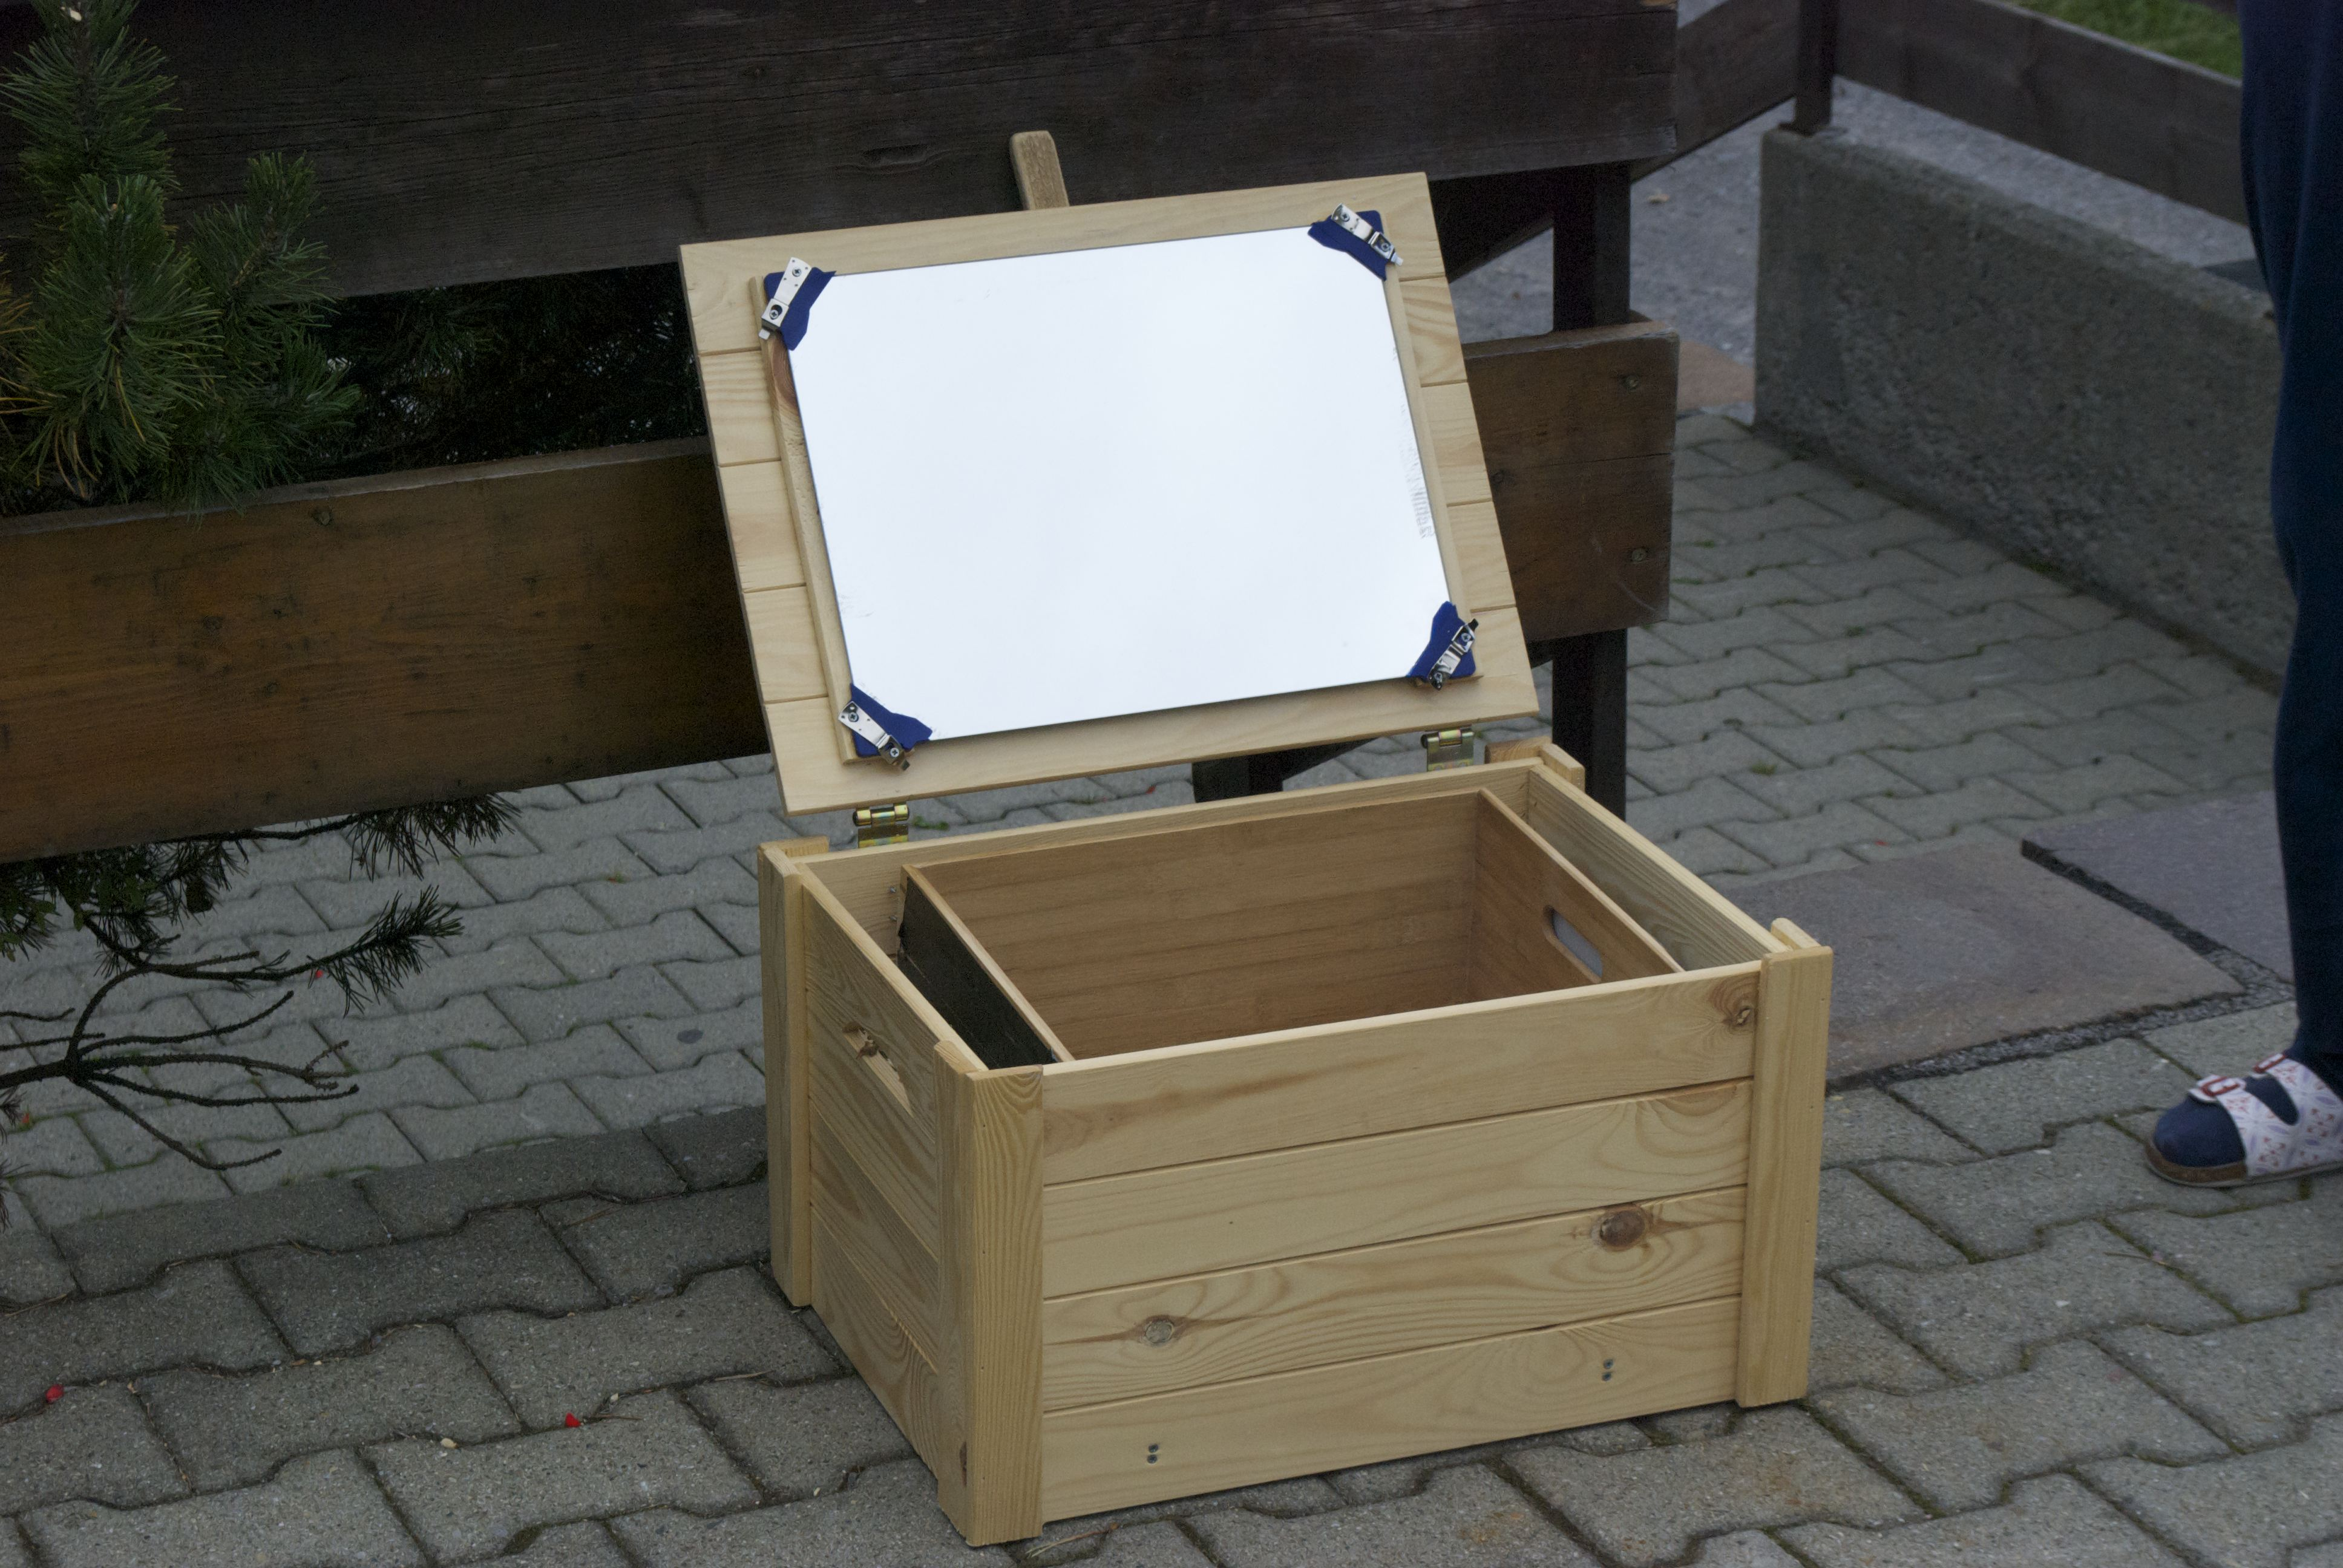
\includegraphics[width=\textwidth]{figs/ofen/DSC_1591}
\end{figure}

Der Solarofen besteht vordergründig aus zwei verschieden großen Holzkisten, wobei die kleinere Holzkiste aus Bambus besteht und auf zwei Holzleisten so innerhalb der großen Holzkiste platziert ist, dass rundherum ca. 3 cm Abstand zur großen Kiste besteht.
Dieser Zwischenraum bleibt wahlweise offen oder wird mit Isoliermaterial befüllt.

\begin{figure}
\centering
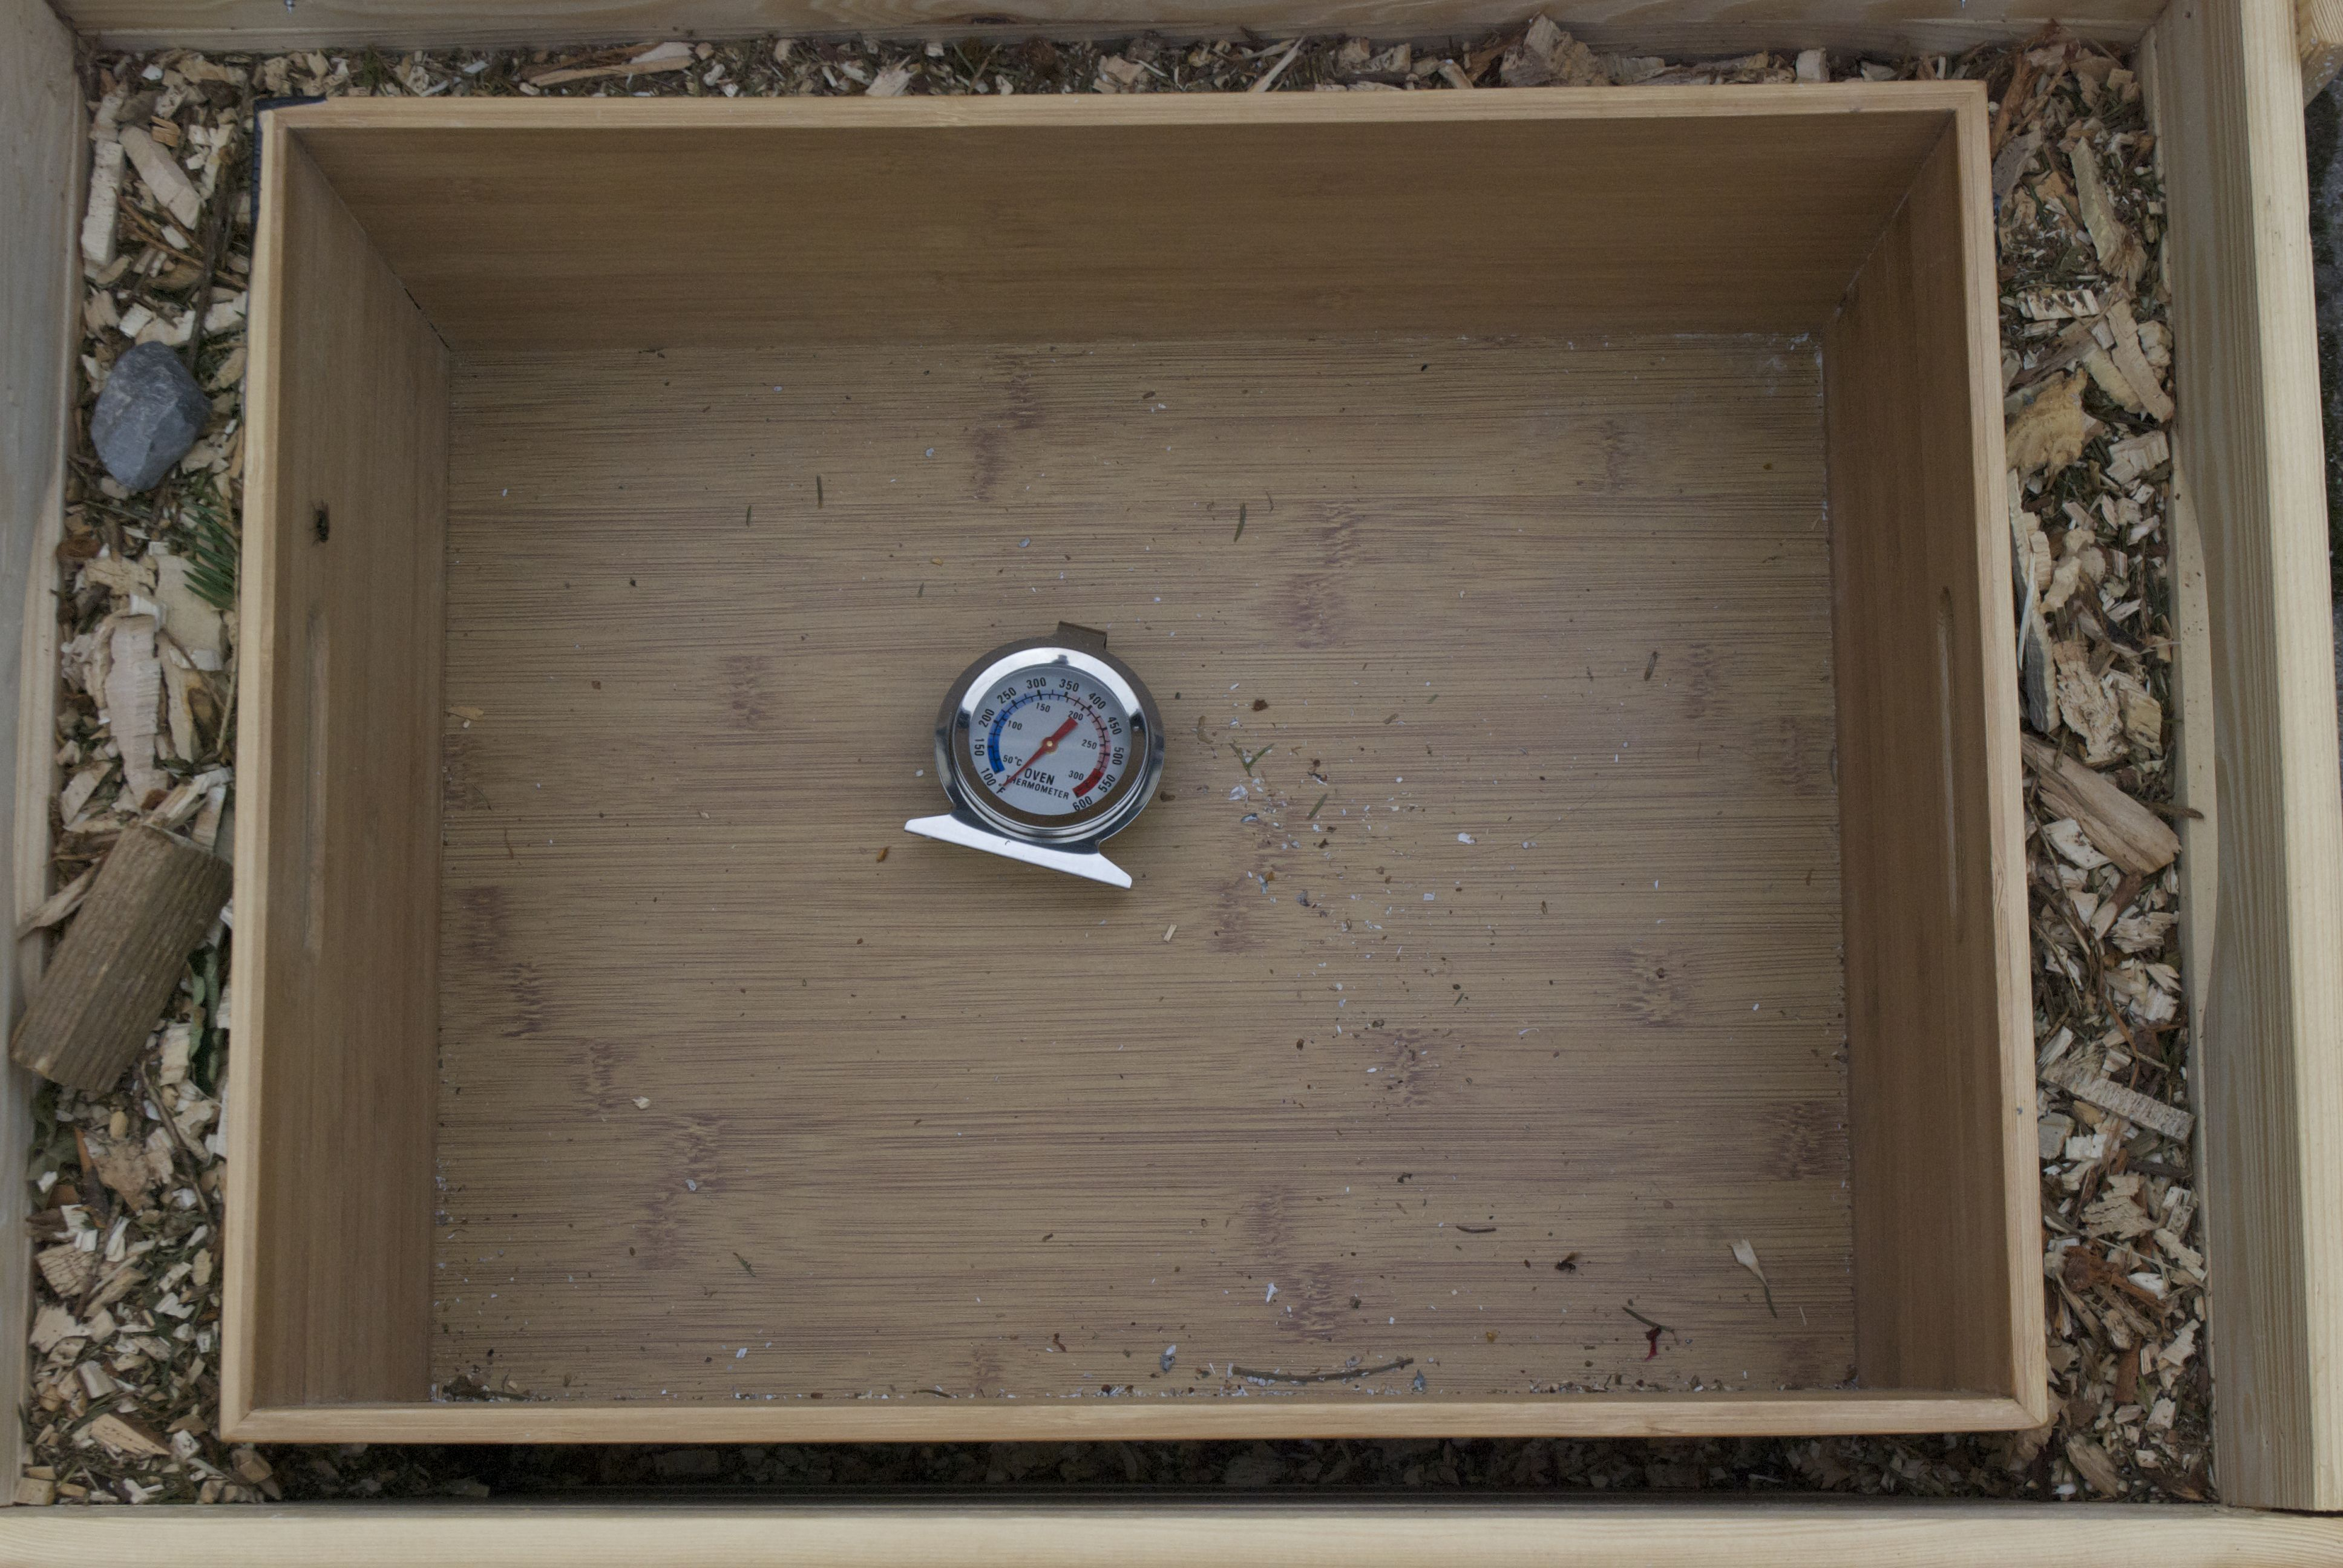
\includegraphics[width=\textwidth]{figs/ofen/DSC_1584}
\end{figure}

Eine Glasscheibe verschließt den in der kleinen Kiste entstandenen Ofenraum lichtdurchlässig.
Diese ist einem handelsüblichen Bilderrahmen entnommen.

Der zur äußeren Holzkiste gehörige Deckel ist über Scharniere beweglich an eben dieser befestigt. Auf der Innenseite des Deckels ist ein als Reflexionsfläche dienender Spiegel angebracht.

Durch Schließen des Deckels wird der Holzofen transportfähig. Ein mit dem Deckel verschraubter Griff erleichtert das Öffnen.

\subsection{Stadien der Konstruktion} 
Das Anbringen des Deckels, der Leisten im Zwischenraum und des Griffes über Schraubverbindungen, sowie das Platzieren der kleineren in der größeren Kiste verlief ohne nennenswerten Aufwand. Benötigt wurden dazu lediglich ein Schraubendreher und ein Dremel mit Trennscheibe.

Da die verwendete Glasscheibe nicht ohne Rückwand im Bilderrahmen hält, musste hier eine alternative Fixierung gesucht werden. Es wurde entschieden, die Ecken der aus Presspappe bestehenden Rückwand im 45$^\circ$-Winkel abzutrennen. Im Rahmen befand sich bereits ein umlaufender Schlitz. Durch Einstecken der Pappwinkel an den Ecken in diesen Schlitz konnte die Scheibe im Rahmen verankert werden. Nachteil dieser Befestigung ist allerdings ein Spalt zwischen innerer Holzkiste und Glasscheibe, durch den prinzipiell warme Luft entweichen kann.

Zum Anbringen des Spiegels auf dem Kistendeckel wurde ein Epoxy-Kleber verwendet. Die Klebeverbindung musste über Nacht aushärten.

Um Grifflöcher in der inneren Kiste zu verschließen, wurde Aluminium, welches von den anderen Arbeiten übrigblieb, und Gewebeband genutzt. 

Um über den Spiegel Sonnenlicht in das Innere des Ofens zu leiten, muss der Spiegel im Deckel im spitzen Winkel zur Kiste gehalten werden. Hierzu hat sich ein Band zwischen Griff im Deckel und einer Bank als Halterung als praktikabel herausgestellt.
  
Als Nächstes wurde Isoliermaterial in den Zwischenraum eingebracht. Das verwendete Isoliermaterial waren gehäckselte Holzabfälle, die eine Zirkulation der Luft verhindert sollten. 

In den folgenden Tagen wurde unter anderem durch Variation des Winkels zwischen Kiste und Untergrund versucht, die Intensität des einfallenden Lichtes zu vergrößern.

Die auf den Spiegel wirkenden Kräfte sorgten nach zwei Tagen dafür, dass sich die Epoxy-Klebeverbindung löste. Verantwortlich dafür war wahrscheinlich die unterschiedliche Ausdehnung der verschiedenen verwandten Materialien.  Daraufhin wurden die Ecken des Spiegels mit aus der Rückwand des Bilderrahmens gewonnenen Metallspangen mit dem Deckel verschraubt.  % Das war ziemlich genial :D

Als Auskleidung des Ofeninnenraums wurde sowohl Aluminium als auch eine schwarze Mülltüte erprobt. 

Zuletzt wurde der Spalt zwischen innerer Holzkiste und Glasscheibe mit einem geflochtenen Band aus Kunstfaser verschlossen.


\subsection{Messungen}
Ein erster Probelauf ohne Isolierung und Innenauskleidung brachte eine Temperatur von ca. $80^\circ$C, die über ein Ofenthermometer im Inneren bestimmt wurde.

Alle weiteren Veränderungen führten nur zu Temperaturen von ca. $40-60^\circ$C. Vermutlich lag dies an dem verwendeten Isoliermaterial, welches die Wärmekapazität des gesamten Ofens erhöhte.

Die Innenverkleidung aus Aluminiumplatten hat keine nennenswerten Veränderungen gebracht. Die Gruppe war sich einig, dass eine schwarze Oberfläche im Ofen allerdings essentiell ist, um möglichst viel Energie des einfallenden Lichts zu absorbieren. Die schwarze Mülltüte als Innenverkleidung bestätigte diese Annahme, da mit ihr $60^\circ$C im Inneren des Ofens gemessen wurden. Diese Temperatur reichte bereits, um die Plastiktüte zum Schmelzen zu bringen. 
Somit hat sich insgesamt weder blankes Aluminium noch Plastik als Innenverkleidung bewährt. Letzlich scheiterte eine Umsetzung der Innenraumverkleidung an fehlenden Materialien. Notwendig wären schwarze Ofenfarbe oder eine hitzebeständige Folie gewesen.

In einer Vergleichsmessung außerhalb des Ofens war die gemessenen Temperatur ca. $50^\circ$C.

Als letzter Versuch wurden zwei rohe Eier über einen Tag im Sonnenofen erwärmt. Eines der beiden Eier wies am Ende leicht gestocktes Eiweiß auf. % Ich wette das waren einfach nur sehr viele Salmonellen

\subsection{Verbesserungen}

Sowohl Material als auch Farbe der Innenauskleidung sollten variiert werden. Dunkle Farben sind aufgrund eines im Allgemeinen mit ihr verbundenen hohen Absorptionskoeffizienten zu bevorzugen. 

Auch das Isoliermaterial in den Zwischenräumen des Solarofens bedarf Verbesserung, insbesondere unter dem Gesichtspunkt, dass es die Wärmekapazität des Ofens nicht verschlechtern darf. Eventuell wäre es vorteilhaft die Isolierung nur durch ein abgeschlossenes Luftvolumen zu realisieren.

Als Feinschliff, der allerdings keinen Einfluss auf die Temperatur des Ofens haben sollte, kann sowohl eine Befestigung der Glasscheibe auf der inneren Kiste konstruiert werden -- diese lag während der Versuche lose auf der Öffnung --, als auch ein Stab zum Offenhalten des Deckels gebaut werden.